\documentclass[twoside]{book}

% Packages required by doxygen
\usepackage{calc}
\usepackage{doxygen}
\usepackage{graphicx}
\usepackage[utf8]{inputenc}
\usepackage{makeidx}
\usepackage{multicol}
\usepackage{multirow}
\usepackage{textcomp}
\usepackage[table]{xcolor}

% Font selection
\usepackage[T1]{fontenc}
\usepackage{mathptmx}
\usepackage[scaled=.90]{helvet}
\usepackage{courier}
\usepackage{amssymb}
\usepackage{sectsty}
\renewcommand{\familydefault}{\sfdefault}
\allsectionsfont{%
  \fontseries{bc}\selectfont%
  \color{darkgray}%
}
\renewcommand{\DoxyLabelFont}{%
  \fontseries{bc}\selectfont%
  \color{darkgray}%
}

% Page & text layout
\usepackage{geometry}
\geometry{%
  a4paper,%
  top=2.5cm,%
  bottom=2.5cm,%
  left=2.5cm,%
  right=2.5cm%
}
\tolerance=750
\hfuzz=15pt
\hbadness=750
\setlength{\emergencystretch}{15pt}
\setlength{\parindent}{0cm}
\setlength{\parskip}{0.2cm}
\makeatletter
\renewcommand{\paragraph}{%
  \@startsection{paragraph}{4}{0ex}{-1.0ex}{1.0ex}{%
    \normalfont\normalsize\bfseries\SS@parafont%
  }%
}
\renewcommand{\subparagraph}{%
  \@startsection{subparagraph}{5}{0ex}{-1.0ex}{1.0ex}{%
    \normalfont\normalsize\bfseries\SS@subparafont%
  }%
}
\makeatother

% Headers & footers
\usepackage{fancyhdr}
\pagestyle{fancyplain}
\fancyhead[LE]{\fancyplain{}{\bfseries\thepage}}
\fancyhead[CE]{\fancyplain{}{}}
\fancyhead[RE]{\fancyplain{}{\bfseries\leftmark}}
\fancyhead[LO]{\fancyplain{}{\bfseries\rightmark}}
\fancyhead[CO]{\fancyplain{}{}}
\fancyhead[RO]{\fancyplain{}{\bfseries\thepage}}
\fancyfoot[LE]{\fancyplain{}{}}
\fancyfoot[CE]{\fancyplain{}{}}
\fancyfoot[RE]{\fancyplain{}{\bfseries\scriptsize Generated on Fri May 27 2016 22\-:27\-:08 for My Project by Doxygen }}
\fancyfoot[LO]{\fancyplain{}{\bfseries\scriptsize Generated on Fri May 27 2016 22\-:27\-:08 for My Project by Doxygen }}
\fancyfoot[CO]{\fancyplain{}{}}
\fancyfoot[RO]{\fancyplain{}{}}
\renewcommand{\footrulewidth}{0.4pt}
\renewcommand{\chaptermark}[1]{%
  \markboth{#1}{}%
}
\renewcommand{\sectionmark}[1]{%
  \markright{\thesection\ #1}%
}

% Indices & bibliography
\usepackage{natbib}
\usepackage[titles]{tocloft}
\setcounter{tocdepth}{3}
\setcounter{secnumdepth}{5}
\makeindex

% Hyperlinks (required, but should be loaded last)
\usepackage{ifpdf}
\ifpdf
  \usepackage[pdftex,pagebackref=true]{hyperref}
\else
  \usepackage[ps2pdf,pagebackref=true]{hyperref}
\fi
\hypersetup{%
  colorlinks=true,%
  linkcolor=blue,%
  citecolor=blue,%
  unicode%
}

% Custom commands
\newcommand{\clearemptydoublepage}{%
  \newpage{\pagestyle{empty}\cleardoublepage}%
}


%===== C O N T E N T S =====

\begin{document}

% Titlepage & ToC
\hypersetup{pageanchor=false}
\pagenumbering{roman}
\begin{titlepage}
\vspace*{7cm}
\begin{center}%
{\Large My Project }\\
\vspace*{1cm}
{\large Generated by Doxygen 1.8.6}\\
\vspace*{0.5cm}
{\small Fri May 27 2016 22:27:08}\\
\end{center}
\end{titlepage}
\clearemptydoublepage
\tableofcontents
\clearemptydoublepage
\pagenumbering{arabic}
\hypersetup{pageanchor=true}

%--- Begin generated contents ---
\chapter{raspberry\-Pi}
\label{md_README}
\hypertarget{md_README}{}
Peripheral Interface on raspberry Pi 
\chapter{File Index}
\section{File List}
Here is a list of all documented files with brief descriptions\-:\begin{DoxyCompactList}
\item\contentsline{section}{\hyperlink{main_8c}{main.\-c} \\*Raspberry Pi is interfaced with M\-C\-P4970\-N(I2\-C-\/\-R\-T\-C from Microchip)

Detailed description of file }{\pageref{main_8c}}{}
\end{DoxyCompactList}

\chapter{File Documentation}
\hypertarget{main_8c}{\section{main.\-c File Reference}
\label{main_8c}\index{main.\-c@{main.\-c}}
}


Raspberry Pi is interfaced with M\-C\-P4970\-N(I2\-C-\/\-R\-T\-C from Microchip)

Detailed description of file.  


{\ttfamily \#include $<$stdio.\-h$>$}\\*
{\ttfamily \#include $<$fcntl.\-h$>$}\\*
{\ttfamily \#include $<$unistd.\-h$>$}\\*
{\ttfamily \#include $<$stdlib.\-h$>$}\\*
{\ttfamily \#include $<$stdint.\-h$>$}\\*
{\ttfamily \#include $<$linux/fs.\-h$>$}\\*
{\ttfamily \#include $<$sys/types.\-h$>$}\\*
{\ttfamily \#include $<$sys/ioctl.\-h$>$}\\*
{\ttfamily \#include $<$errno.\-h$>$}\\*
{\ttfamily \#include $<$assert.\-h$>$}\\*
{\ttfamily \#include $<$string.\-h$>$}\\*
{\ttfamily \#include $<$getopt.\-h$>$}\\*
{\ttfamily \#include $<$sys/stat.\-h$>$}\\*
{\ttfamily \#include $<$linux/i2c-\/dev.\-h$>$}\\*
{\ttfamily \#include $<$linux/i2c.\-h$>$}\\*
Include dependency graph for main.\-c\-:\nopagebreak
\begin{figure}[H]
\begin{center}
\leavevmode
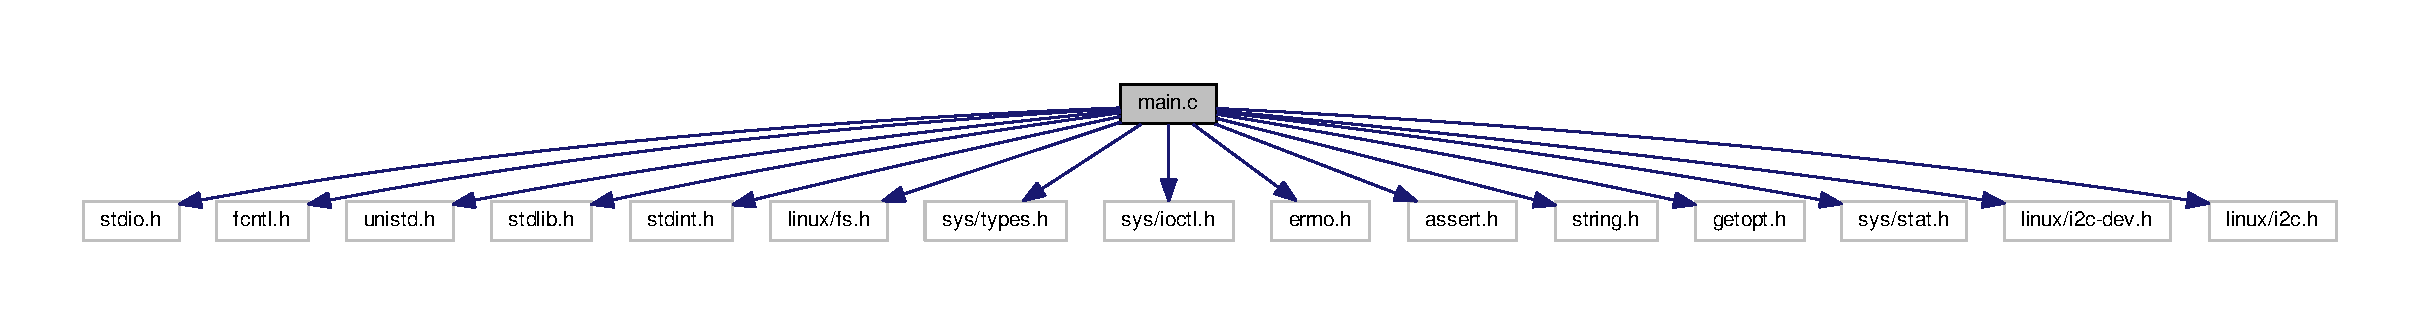
\includegraphics[width=350pt]{main_8c__incl}
\end{center}
\end{figure}
\subsection*{Macros}
\begin{DoxyCompactItemize}
\item 
\hypertarget{main_8c_a7c5d1c7f4a102bc090361b840c211815}{\#define \hyperlink{main_8c_a7c5d1c7f4a102bc090361b840c211815}{R\-T\-C\-\_\-\-A\-D\-D\-R\-E\-S\-S}~0x6\-F}\label{main_8c_a7c5d1c7f4a102bc090361b840c211815}

\begin{DoxyCompactList}\small\item\em 0b01101111 \end{DoxyCompactList}\item 
\hypertarget{main_8c_a9e1b4f5aa30a371cbec0d87aab0c569d}{\#define \hyperlink{main_8c_a9e1b4f5aa30a371cbec0d87aab0c569d}{A\-D\-D\-R\-\_\-\-S\-E\-C}~0x00}\label{main_8c_a9e1b4f5aa30a371cbec0d87aab0c569d}

\begin{DoxyCompactList}\small\item\em address of S\-E\-C\-O\-N\-D\-S register \end{DoxyCompactList}\item 
\hypertarget{main_8c_a73d3f328999be0d2dd7ba991280b342e}{\#define \hyperlink{main_8c_a73d3f328999be0d2dd7ba991280b342e}{A\-D\-D\-R\-\_\-\-M\-I\-N}~0x01}\label{main_8c_a73d3f328999be0d2dd7ba991280b342e}

\begin{DoxyCompactList}\small\item\em address of M\-I\-N\-U\-T\-E\-S register \end{DoxyCompactList}\item 
\hypertarget{main_8c_aea073397d3f8ed0bc081263118fab6c6}{\#define \hyperlink{main_8c_aea073397d3f8ed0bc081263118fab6c6}{A\-D\-D\-R\-\_\-\-H\-O\-U\-R}~0x02}\label{main_8c_aea073397d3f8ed0bc081263118fab6c6}

\begin{DoxyCompactList}\small\item\em address of H\-O\-U\-R\-S register \end{DoxyCompactList}\item 
\hypertarget{main_8c_a00c8fd570087116240d11a59587956ec}{\#define \hyperlink{main_8c_a00c8fd570087116240d11a59587956ec}{A\-D\-D\-R\-\_\-\-D\-A\-Y}~0x03}\label{main_8c_a00c8fd570087116240d11a59587956ec}

\begin{DoxyCompactList}\small\item\em address of D\-A\-Y O\-F W\-K register \end{DoxyCompactList}\item 
\hypertarget{main_8c_a9be8fc8df9943f7b31c16bef0b187b12}{\#define \hyperlink{main_8c_a9be8fc8df9943f7b31c16bef0b187b12}{A\-D\-D\-R\-\_\-\-S\-T\-A\-T}~0x03}\label{main_8c_a9be8fc8df9943f7b31c16bef0b187b12}

\begin{DoxyCompactList}\small\item\em address of S\-T\-A\-T\-U\-S register \end{DoxyCompactList}\item 
\hypertarget{main_8c_a46f0766436c6b5936ecb451f2577c4e0}{\#define \hyperlink{main_8c_a46f0766436c6b5936ecb451f2577c4e0}{A\-D\-D\-R\-\_\-\-D\-A\-T\-E}~0x04}\label{main_8c_a46f0766436c6b5936ecb451f2577c4e0}

\begin{DoxyCompactList}\small\item\em address of D\-A\-T\-E register \end{DoxyCompactList}\item 
\hypertarget{main_8c_afb97f3475c8c3a7492edc7945750666f}{\#define \hyperlink{main_8c_afb97f3475c8c3a7492edc7945750666f}{A\-D\-D\-R\-\_\-\-M\-N\-T\-H}~0x05}\label{main_8c_afb97f3475c8c3a7492edc7945750666f}

\begin{DoxyCompactList}\small\item\em address of M\-O\-N\-T\-H register \end{DoxyCompactList}\item 
\hypertarget{main_8c_a82817248c68d8c1a20bfd925f801dbf2}{\#define \hyperlink{main_8c_a82817248c68d8c1a20bfd925f801dbf2}{A\-D\-D\-R\-\_\-\-Y\-E\-A\-R}~0x06}\label{main_8c_a82817248c68d8c1a20bfd925f801dbf2}

\begin{DoxyCompactList}\small\item\em address of Y\-E\-A\-R register \end{DoxyCompactList}\item 
\hypertarget{main_8c_a2fde73f3515eba84d807f4fe03d0de0f}{\#define \hyperlink{main_8c_a2fde73f3515eba84d807f4fe03d0de0f}{A\-D\-D\-R\-\_\-\-C\-T\-R\-L}~0x07}\label{main_8c_a2fde73f3515eba84d807f4fe03d0de0f}

\begin{DoxyCompactList}\small\item\em address of C\-O\-N\-T\-R\-O\-L register \end{DoxyCompactList}\item 
\hypertarget{main_8c_a2b0a079c4a29f0f5d3a9fa78805479dc}{\#define \hyperlink{main_8c_a2b0a079c4a29f0f5d3a9fa78805479dc}{A\-D\-D\-R\-\_\-\-C\-A\-L}~0x08}\label{main_8c_a2b0a079c4a29f0f5d3a9fa78805479dc}

\begin{DoxyCompactList}\small\item\em address of C\-A\-L\-I\-B register \end{DoxyCompactList}\item 
\hypertarget{main_8c_aa407647356df189135b1ed15174460b4}{\#define \hyperlink{main_8c_aa407647356df189135b1ed15174460b4}{A\-D\-D\-R\-\_\-\-U\-L\-I\-D}~0x09}\label{main_8c_aa407647356df189135b1ed15174460b4}

\begin{DoxyCompactList}\small\item\em address of U\-N\-L\-O\-C\-K I\-D register \end{DoxyCompactList}\item 
\hypertarget{main_8c_aa1aca1b5a378fd8d4a18b2d44f78de7a}{\#define \hyperlink{main_8c_aa1aca1b5a378fd8d4a18b2d44f78de7a}{S\-T\-A\-R\-T\-\_\-32\-K\-H\-Z}~0x80}\label{main_8c_aa1aca1b5a378fd8d4a18b2d44f78de7a}

\begin{DoxyCompactList}\small\item\em start crystal\-: S\-T = b7 (A\-D\-D\-R\-\_\-\-S\-E\-C) \end{DoxyCompactList}\item 
\hypertarget{main_8c_a5b11d088a6ab6484ad47eaa4398e58eb}{\#define \hyperlink{main_8c_a5b11d088a6ab6484ad47eaa4398e58eb}{L\-P}~0x20}\label{main_8c_a5b11d088a6ab6484ad47eaa4398e58eb}

\begin{DoxyCompactList}\small\item\em mask for the leap year bit(\-M\-O\-N\-T\-H R\-E\-G) \end{DoxyCompactList}\item 
\hypertarget{main_8c_a2209a3a4f13b898b3202f70840eaad85}{\#define \hyperlink{main_8c_a2209a3a4f13b898b3202f70840eaad85}{H\-O\-U\-R\-\_\-12}~0x40}\label{main_8c_a2209a3a4f13b898b3202f70840eaad85}

\begin{DoxyCompactList}\small\item\em 12 hours format (A\-D\-D\-R\-\_\-\-H\-O\-U\-R) \end{DoxyCompactList}\item 
\hypertarget{main_8c_a23c7d58108d99a089ce0824823e6b950}{\#define \hyperlink{main_8c_a23c7d58108d99a089ce0824823e6b950}{P\-M}~0x20}\label{main_8c_a23c7d58108d99a089ce0824823e6b950}

\begin{DoxyCompactList}\small\item\em post-\/meridian bit (A\-D\-D\-R\-\_\-\-H\-O\-U\-R) \end{DoxyCompactList}\item 
\hypertarget{main_8c_a4077bef57f7b230360d3c9fd61abe7b7}{\#define \hyperlink{main_8c_a4077bef57f7b230360d3c9fd61abe7b7}{O\-U\-T\-\_\-\-P\-I\-N}~0x80}\label{main_8c_a4077bef57f7b230360d3c9fd61abe7b7}

\begin{DoxyCompactList}\small\item\em = b7 (A\-D\-D\-R\-\_\-\-C\-T\-R\-L) \end{DoxyCompactList}\item 
\hypertarget{main_8c_a3eb471417c5e9c54468288c45c6d138b}{\#define \hyperlink{main_8c_a3eb471417c5e9c54468288c45c6d138b}{S\-Q\-W\-E}~0x40}\label{main_8c_a3eb471417c5e9c54468288c45c6d138b}

\begin{DoxyCompactList}\small\item\em S\-Q\-W\-E = b6 (A\-D\-D\-R\-\_\-\-C\-T\-R\-L) \end{DoxyCompactList}\item 
\hypertarget{main_8c_ae22568886152d2c16996fcbf8151fc4c}{\#define \hyperlink{main_8c_ae22568886152d2c16996fcbf8151fc4c}{A\-L\-M\-\_\-\-N\-O}~0x00}\label{main_8c_ae22568886152d2c16996fcbf8151fc4c}

\begin{DoxyCompactList}\small\item\em no alarm activated (A\-D\-D\-R\-\_\-\-C\-T\-R\-L) \end{DoxyCompactList}\item 
\hypertarget{main_8c_ab11e8e43069fb6fb23f561395a651d6b}{\#define \hyperlink{main_8c_ab11e8e43069fb6fb23f561395a651d6b}{A\-L\-M\-\_\-0}~0x10}\label{main_8c_ab11e8e43069fb6fb23f561395a651d6b}

\begin{DoxyCompactList}\small\item\em A\-L\-A\-R\-M0 is activated (A\-D\-D\-R\-\_\-\-C\-T\-R\-L) \end{DoxyCompactList}\item 
\hypertarget{main_8c_a8884f97037d39bbfbd83208c62f447a7}{\#define \hyperlink{main_8c_a8884f97037d39bbfbd83208c62f447a7}{A\-L\-M\-\_\-1}~0x20}\label{main_8c_a8884f97037d39bbfbd83208c62f447a7}

\begin{DoxyCompactList}\small\item\em A\-L\-A\-R\-M1 is activated (A\-D\-D\-R\-\_\-\-C\-T\-R\-L) \end{DoxyCompactList}\item 
\hypertarget{main_8c_a813537cf38515e9f2877185ffc0236c9}{\#define \hyperlink{main_8c_a813537cf38515e9f2877185ffc0236c9}{A\-L\-M\-\_\-01}~0x30}\label{main_8c_a813537cf38515e9f2877185ffc0236c9}

\begin{DoxyCompactList}\small\item\em both alarms are activated (A\-D\-D\-R\-\_\-\-C\-T\-R\-L) \end{DoxyCompactList}\item 
\hypertarget{main_8c_a78b153a51ee9abd06f5b720ecfcad853}{\#define \hyperlink{main_8c_a78b153a51ee9abd06f5b720ecfcad853}{M\-F\-P\-\_\-01\-H}~0x00}\label{main_8c_a78b153a51ee9abd06f5b720ecfcad853}

\begin{DoxyCompactList}\small\item\em M\-F\-P = S\-Q\-V\-A\-W(01 H\-E\-R\-Z) (A\-D\-D\-R\-\_\-\-C\-T\-R\-L) \end{DoxyCompactList}\item 
\hypertarget{main_8c_af64218da50241dc41d5c85965a0421ab}{\#define \hyperlink{main_8c_af64218da50241dc41d5c85965a0421ab}{M\-F\-P\-\_\-04\-K}~0x01}\label{main_8c_af64218da50241dc41d5c85965a0421ab}

\begin{DoxyCompactList}\small\item\em M\-F\-P = S\-Q\-V\-A\-W(04 K\-H\-Z) (A\-D\-D\-R\-\_\-\-C\-T\-R\-L) \end{DoxyCompactList}\item 
\hypertarget{main_8c_a852aa86e888d78386a858d8d717c0d57}{\#define \hyperlink{main_8c_a852aa86e888d78386a858d8d717c0d57}{M\-F\-P\-\_\-08\-K}~0x02}\label{main_8c_a852aa86e888d78386a858d8d717c0d57}

\begin{DoxyCompactList}\small\item\em M\-F\-P = S\-Q\-V\-A\-W(08 K\-H\-Z) (A\-D\-D\-R\-\_\-\-C\-T\-R\-L) \end{DoxyCompactList}\item 
\hypertarget{main_8c_aa8d3db894547e9638f98723c4ecf85e2}{\#define \hyperlink{main_8c_aa8d3db894547e9638f98723c4ecf85e2}{M\-F\-P\-\_\-32\-K}~0x03}\label{main_8c_aa8d3db894547e9638f98723c4ecf85e2}

\begin{DoxyCompactList}\small\item\em M\-F\-P = S\-Q\-V\-A\-W(32 K\-H\-Z) (A\-D\-D\-R\-\_\-\-C\-T\-R\-L) \end{DoxyCompactList}\item 
\hypertarget{main_8c_abc98d564eb40283898c37f8fb6608321}{\#define \hyperlink{main_8c_abc98d564eb40283898c37f8fb6608321}{M\-F\-P\-\_\-64\-H}~0x04}\label{main_8c_abc98d564eb40283898c37f8fb6608321}

\begin{DoxyCompactList}\small\item\em M\-F\-P = S\-Q\-V\-A\-W(64 H\-E\-R\-Z) (A\-D\-D\-R\-\_\-\-C\-T\-R\-L) \end{DoxyCompactList}\item 
\hypertarget{main_8c_aa0d5ebd28cc8fd3c9ad899677649cc72}{\#define \hyperlink{main_8c_aa0d5ebd28cc8fd3c9ad899677649cc72}{A\-L\-Mx\-\_\-\-P\-O\-L}~0x80}\label{main_8c_aa0d5ebd28cc8fd3c9ad899677649cc72}

\begin{DoxyCompactList}\small\item\em polarity of M\-F\-P on alarm (A\-D\-D\-R\-\_\-\-A\-L\-Mx\-C\-T\-L) \end{DoxyCompactList}\item 
\hypertarget{main_8c_a9918cc026eb3bd51262d7162f140d3cf}{\#define \hyperlink{main_8c_a9918cc026eb3bd51262d7162f140d3cf}{A\-L\-Mx\-C\-\_\-\-S\-E\-C}~0x00}\label{main_8c_a9918cc026eb3bd51262d7162f140d3cf}

\begin{DoxyCompactList}\small\item\em A\-L\-A\-R\-M compare on S\-E\-C (A\-D\-D\-R\-\_\-\-A\-L\-Mx\-C\-T\-L) \end{DoxyCompactList}\item 
\hypertarget{main_8c_a5c16ca3ab7d2b1accdc09023dda2c55d}{\#define \hyperlink{main_8c_a5c16ca3ab7d2b1accdc09023dda2c55d}{A\-L\-Mx\-C\-\_\-\-M\-I\-N}~0x10}\label{main_8c_a5c16ca3ab7d2b1accdc09023dda2c55d}

\begin{DoxyCompactList}\small\item\em A\-L\-A\-R\-M compare on M\-I\-N (A\-D\-D\-R\-\_\-\-A\-L\-Mx\-C\-T\-L) \end{DoxyCompactList}\item 
\hypertarget{main_8c_a781bb8634d05e8076c9f93b2726a205b}{\#define \hyperlink{main_8c_a781bb8634d05e8076c9f93b2726a205b}{A\-L\-Mx\-C\-\_\-\-H\-R}~0x20}\label{main_8c_a781bb8634d05e8076c9f93b2726a205b}

\begin{DoxyCompactList}\small\item\em A\-L\-A\-R\-M compare on H\-O\-U\-R (A\-D\-D\-R\-\_\-\-A\-L\-Mx\-C\-T\-L) \end{DoxyCompactList}\item 
\hypertarget{main_8c_a128ce9f8cadf391c1d8c6c9811bb5276}{\#define \hyperlink{main_8c_a128ce9f8cadf391c1d8c6c9811bb5276}{A\-L\-Mx\-C\-\_\-\-D\-A\-Y}~0x30}\label{main_8c_a128ce9f8cadf391c1d8c6c9811bb5276}

\begin{DoxyCompactList}\small\item\em A\-L\-A\-R\-M compare on D\-A\-Y (A\-D\-D\-R\-\_\-\-A\-L\-Mx\-C\-T\-L) \end{DoxyCompactList}\item 
\hypertarget{main_8c_ab83ed7b6b422a4e0da2eef33f2d32e12}{\#define \hyperlink{main_8c_ab83ed7b6b422a4e0da2eef33f2d32e12}{A\-L\-Mx\-C\-\_\-\-D\-A\-T}~0x40}\label{main_8c_ab83ed7b6b422a4e0da2eef33f2d32e12}

\begin{DoxyCompactList}\small\item\em A\-L\-A\-R\-M compare on D\-A\-T\-E (A\-D\-D\-R\-\_\-\-A\-L\-Mx\-C\-T\-L) \end{DoxyCompactList}\item 
\hypertarget{main_8c_a3189ddfd38f3fded500b82ead03f0fea}{\#define \hyperlink{main_8c_a3189ddfd38f3fded500b82ead03f0fea}{A\-L\-Mx\-C\-\_\-\-A\-L\-L}~0x70}\label{main_8c_a3189ddfd38f3fded500b82ead03f0fea}

\begin{DoxyCompactList}\small\item\em A\-L\-A\-R\-M compare on all param(\-A\-D\-D\-R\-\_\-\-A\-L\-Mx\-C\-T\-L) \end{DoxyCompactList}\item 
\hypertarget{main_8c_a082f652bf03af20b93ffa1674b414491}{\#define \hyperlink{main_8c_a082f652bf03af20b93ffa1674b414491}{A\-L\-Mx\-\_\-\-I\-F}~0x08}\label{main_8c_a082f652bf03af20b93ffa1674b414491}

\begin{DoxyCompactList}\small\item\em M\-A\-S\-K of the A\-L\-A\-R\-M\-\_\-\-I\-F (A\-D\-D\-R\-\_\-\-A\-L\-Mx\-C\-T\-L) \end{DoxyCompactList}\item 
\hypertarget{main_8c_a5380ef70909a9fcd46fe65e606bfee43}{\#define \hyperlink{main_8c_a5380ef70909a9fcd46fe65e606bfee43}{O\-S\-C\-O\-N}~0x20}\label{main_8c_a5380ef70909a9fcd46fe65e606bfee43}

\begin{DoxyCompactList}\small\item\em state of the oscillator(running or not) \end{DoxyCompactList}\item 
\hypertarget{main_8c_a0a70ffb498fad5a2a5ed1ef1e71ae58c}{\#define \hyperlink{main_8c_a0a70ffb498fad5a2a5ed1ef1e71ae58c}{V\-B\-A\-T\-E\-N}~0x08}\label{main_8c_a0a70ffb498fad5a2a5ed1ef1e71ae58c}

\begin{DoxyCompactList}\small\item\em enable battery for back-\/up \end{DoxyCompactList}\end{DoxyCompactItemize}
\subsection*{Functions}
\begin{DoxyCompactItemize}
\item 
\hypertarget{main_8c_ac61ef6fe48369f69d5b35df0bccfcde0}{int {\bfseries i2\-C\-Setup\-Device} (const char $\ast$dev\-Bus, int dev\-Address)}\label{main_8c_ac61ef6fe48369f69d5b35df0bccfcde0}

\item 
\hypertarget{main_8c_ae66f6b31b5ad750f1fe042a706a4e3d4}{int {\bfseries main} ()}\label{main_8c_ae66f6b31b5ad750f1fe042a706a4e3d4}

\end{DoxyCompactItemize}


\subsection{Detailed Description}
Raspberry Pi is interfaced with M\-C\-P4970\-N(I2\-C-\/\-R\-T\-C from Microchip)

Detailed description of file. Ankit (\href{mailto:ankit4970@gmail.com}{\tt ankit4970@gmail.\-com}) \begin{DoxyDate}{Date}
May 27, 2016 
\end{DoxyDate}

%--- End generated contents ---

% Index
\newpage
\phantomsection
\addcontentsline{toc}{chapter}{Index}
\printindex

\end{document}
